\documentclass[11pt,a4paper]{article}
\usepackage[T1]{fontenc}
\usepackage[utf8]{inputenc}
\usepackage{lmodern}
\usepackage[margin=2.3cm]{geometry}
\usepackage{graphicx}
\graphicspath{{../img/}}
\usepackage{xcolor}
\definecolor{spblue}{HTML}{1F4E79}
\definecolor{spteal}{HTML}{2C7A7B}
\usepackage{booktabs}
\usepackage{longtable}
\usepackage{array}
\usepackage{enumitem}
\usepackage{float}
\usepackage{caption}
\captionsetup{font=small,labelfont=bf}
\usepackage{listings}
\lstset{basicstyle=\ttfamily\footnotesize,breaklines=true,frame=single,backgroundcolor=\color{gray!8},columns=fullflexible,keepspaces=true}
\usepackage[hidelinks]{hyperref}
\usepackage{titlesec}
\titleformat{\section}{\color{spblue}\Large\bfseries}{\thesection}{0.6em}{}
\titleformat{\subsection}{\color{spteal}\large\bfseries}{\thesubsection}{0.6em}{}
\setlength{\parskip}{0.5em}\setlength{\parindent}{0pt}

\title{ScholarPath --- Class Diagrams\\\large UML Object Model \& Architecture}
\author{ScholarPath Team}
\date{}

\begin{document}
\maketitle

\begin{abstract}
This is Part~4 --- the final instalment --- of a four-part teaching series that
walks the ScholarPath data model from a plain Entity--Relationship Diagram (ERD)
through an Enhanced ER (EERD), then a Relational Mapping, and finally to the
object-oriented design presented here. Where Part~3 produced normalised
\emph{tables}, this document presents the \emph{classes} that those tables
become at run time: the C\# domain entities of the ScholarPath back-end. We
explain why a UML class diagram is the right lens for an object-oriented
codebase, fix a precise notation legend, establish the inheritance foundation
(\texttt{BaseEntity} $\rightarrow$ \texttt{AuditableEntity}, the
\texttt{ISoftDeletable} interface, and the special case of
\texttt{ApplicationUser}), then tour the domain cluster by cluster. We close on
the architectural class view --- the Clean Architecture \emph{ports and
adapters} seam --- which shows how the Application layer depends only on
interfaces while the Infrastructure layer supplies swappable implementations.
Every entity, attribute, and association named here is grounded in the actual
source tree (\texttt{server/src/ScholarPath.Domain/Entities/*} and
\texttt{ScholarPath.Application/Common/Interfaces/*}).
\end{abstract}

\tableofcontents

\section{From the Relational Schema to the Object Model}

\subsection{Why a class diagram?}

Parts~1--3 of this series modelled ScholarPath as \emph{data}: entities,
relationships, and finally relational tables with primary and foreign keys. That
view is correct, but it is incomplete for a system that is \emph{written} in an
object-oriented language. The ScholarPath back-end is built on .NET~10 / C\#,
where the persistent data does not live as bare rows; it lives as
\emph{objects} --- instances of domain classes that carry both state
(attributes) and behaviour (operations). Entity Framework Core then maps those
classes onto the relational tables produced in Part~3. The class diagram is the
bridge: it is the design artefact that the code actually realises.

A UML class diagram answers questions the ERD cannot. It distinguishes
\emph{inheritance} (an \texttt{AuditableEntity} \emph{is a} \texttt{BaseEntity})
from \emph{association} (a \texttt{ConsultantBooking} \emph{references} an
\texttt{ApplicationUser}). It distinguishes a \emph{whole/part} relationship
where the part dies with the whole (composition) from one where the part lives
independently (aggregation). And it lets us model \emph{interfaces} ---
contracts with no data of their own --- which have no equivalent in a pure
relational schema but are central to how ScholarPath stays testable and
provider-agnostic. The diagrams in this document are authored in the style of
\emph{Sommerville, Software Engineering (9th ed.)} and rendered both as Mermaid
\texttt{classDiagram} views and as vector PlantUML PDFs.

\subsection{UML notation legend}

The following notation is used consistently across every figure in this
document. Reading it once here makes the rest of the diagrams self-explanatory.

\begin{table}[H]\centering
\caption{UML class-diagram notation used throughout this document.}
\label{tab:legend}
\small
\begin{tabular}{@{}l l p{8.2cm}@{}}
\toprule
\textbf{UML element} & \textbf{Glyph} & \textbf{Meaning in ScholarPath} \\
\midrule
Generalization & \texttt{Base <|-- Derived} & Inheritance: the derived class
\emph{is a} kind of the base (e.g.\ \texttt{AuditableEntity} $\leftarrow$
\texttt{Scholarship}). Hollow triangle points at the parent. \\
Realization & \texttt{Iface <|.. Class} & A class \emph{implements} an
interface (port). Dashed line, hollow triangle (e.g.\
\texttt{StripeService} realizes \texttt{IStripeService}). \\
Composition & \texttt{Whole *-- Part} & The part cannot exist without the
whole; filled diamond at the whole. Deleting the whole deletes the parts
(e.g.\ \texttt{ChatConversation *-- ChatMessage}). \\
Aggregation & \texttt{Whole o-- Part} & A weaker whole/part link; the part can
outlive the whole. Hollow diamond (e.g.\ \texttt{Payout o-- Payment}). \\
Association & \texttt{A "1" --> "*" B} & A plain reference with role names and
multiplicities at each end (one-to-one, one-to-many, many-to-many). \\
Stereotype & \texttt{<<abstract>>}, \texttt{<<interface>>} & Marks an abstract
base class, an interface (port), or a junction table. \\
\bottomrule
\end{tabular}
\end{table}

Multiplicities are read at the far end of the line: \texttt{A "1" --> "*" B}
means one \texttt{A} is associated with many \texttt{B}, and a \texttt{0..1}
end denotes an optional reference.

\section{The Domain Foundation: Inheritance and the Soft-Delete Contract}

Before the individual entities make sense, three foundational types must be
understood, because almost every other class is defined in terms of them.

\subsection{\texttt{BaseEntity} $\rightarrow$ \texttt{AuditableEntity}}

\texttt{BaseEntity} is the abstract root of the domain. It carries the identity
of every persistent object --- a \texttt{Guid Id} --- and the domain-event
plumbing: a read-only \texttt{DomainEvents} collection plus
\texttt{RaiseDomainEvent(e)} and \texttt{ClearDomainEvents()} operations. This
lets an entity record that something significant happened (for example, a
booking was confirmed) without knowing who will handle it; MediatR dispatches
those events after the unit of work commits.

\texttt{AuditableEntity} is an abstract class that generalizes
\texttt{BaseEntity} and adds the audit and concurrency columns that Part~3
showed on nearly every table: \texttt{CreatedAt}, \texttt{CreatedByUserId},
\texttt{UpdatedAt}, \texttt{UpdatedByUserId}, and a \texttt{RowVersion}
optimistic-concurrency token. The overwhelming majority of ScholarPath's
business entities --- \texttt{Scholarship}, \texttt{ApplicationTracker},
\texttt{UserProfile}, \texttt{Document}, \texttt{ConsultantBooking},
\texttt{Payment}, and so on --- generalize \texttt{AuditableEntity}, which is
exactly why the relational mapping in Part~3 repeated those five audit columns
on table after table. Inheritance in the object model explains the apparent
duplication in the schema.

\subsection{The \texttt{ISoftDeletable} interface}

\texttt{ISoftDeletable} is an \texttt{<<interface>>}: a behavioural contract with
no data of its own that declares the soft-delete state --- \texttt{IsDeleted},
\texttt{DeletedAt}, and \texttt{DeletedByUserId}. Entities that realize it are
never physically removed; instead a global EF~Core query filter hides them. This
is the object-model counterpart of the soft-delete columns and filtered indexes
discussed in Part~3. The class diagrams draw the realization on a representative
subset for legibility, but the contract is realized far more widely --- in
addition to \texttt{ApplicationUser}, \texttt{Scholarship}, and
\texttt{ApplicationTracker}, it is realized by \texttt{Document},
\texttt{CompanyReview} and \texttt{CompanyReviewRequest},
\texttt{ConsultantReview}, \texttt{ConsultantAvailability},
\texttt{ConsultantBooking}, \texttt{Payment}, \texttt{ChatMessage},
\texttt{ForumPost}, \texttt{Resource}, \texttt{Notification},
\texttt{SessionRecording}, and \texttt{SuccessStory}, among others.

\subsection{The special case: \texttt{ApplicationUser} extends ASP.NET Identity}

There is one deliberate and important exception to the inheritance hierarchy.
\texttt{ApplicationUser} does \textbf{not} extend \texttt{BaseEntity} or
\texttt{AuditableEntity}. It extends ASP.NET Core Identity's
\texttt{IdentityUser<Guid>}, and \texttt{ApplicationRole} extends
\texttt{IdentityRole<Guid>}. This is required so that the framework's
authentication, password-hashing, lockout, and role machinery operate on the
user class directly. The trade-off is that, because C\# is single-inheritance,
\texttt{ApplicationUser} cannot also inherit \texttt{BaseEntity}; it therefore
re-implements the domain-event plumbing manually and realizes
\texttt{ISoftDeletable} on its own. Beyond the Identity members it adds the
ScholarPath-specific fields \texttt{Email}, \texttt{FirstName},
\texttt{LastName}, an \texttt{AccountStatus}, the multi-role \texttt{ActiveRole}
selector, \texttt{IsOnboardingComplete}, and a \texttt{FullName()} operation.
Recognising this exception is essential when reading the schema: the
\texttt{AspNetUsers} table is shaped by Identity, not by the ScholarPath base
classes.

\section{The Domain Model, Cluster by Cluster}

Figure~\ref{fig:domain} presents the full domain model on one canvas --- every
business entity, its generalization to the base types, and the principal
associations between clusters. The subsections that follow zoom into each
cluster so the multiplicities and the composition-versus-aggregation choices can
be read clearly.

\begin{figure}[H]\centering
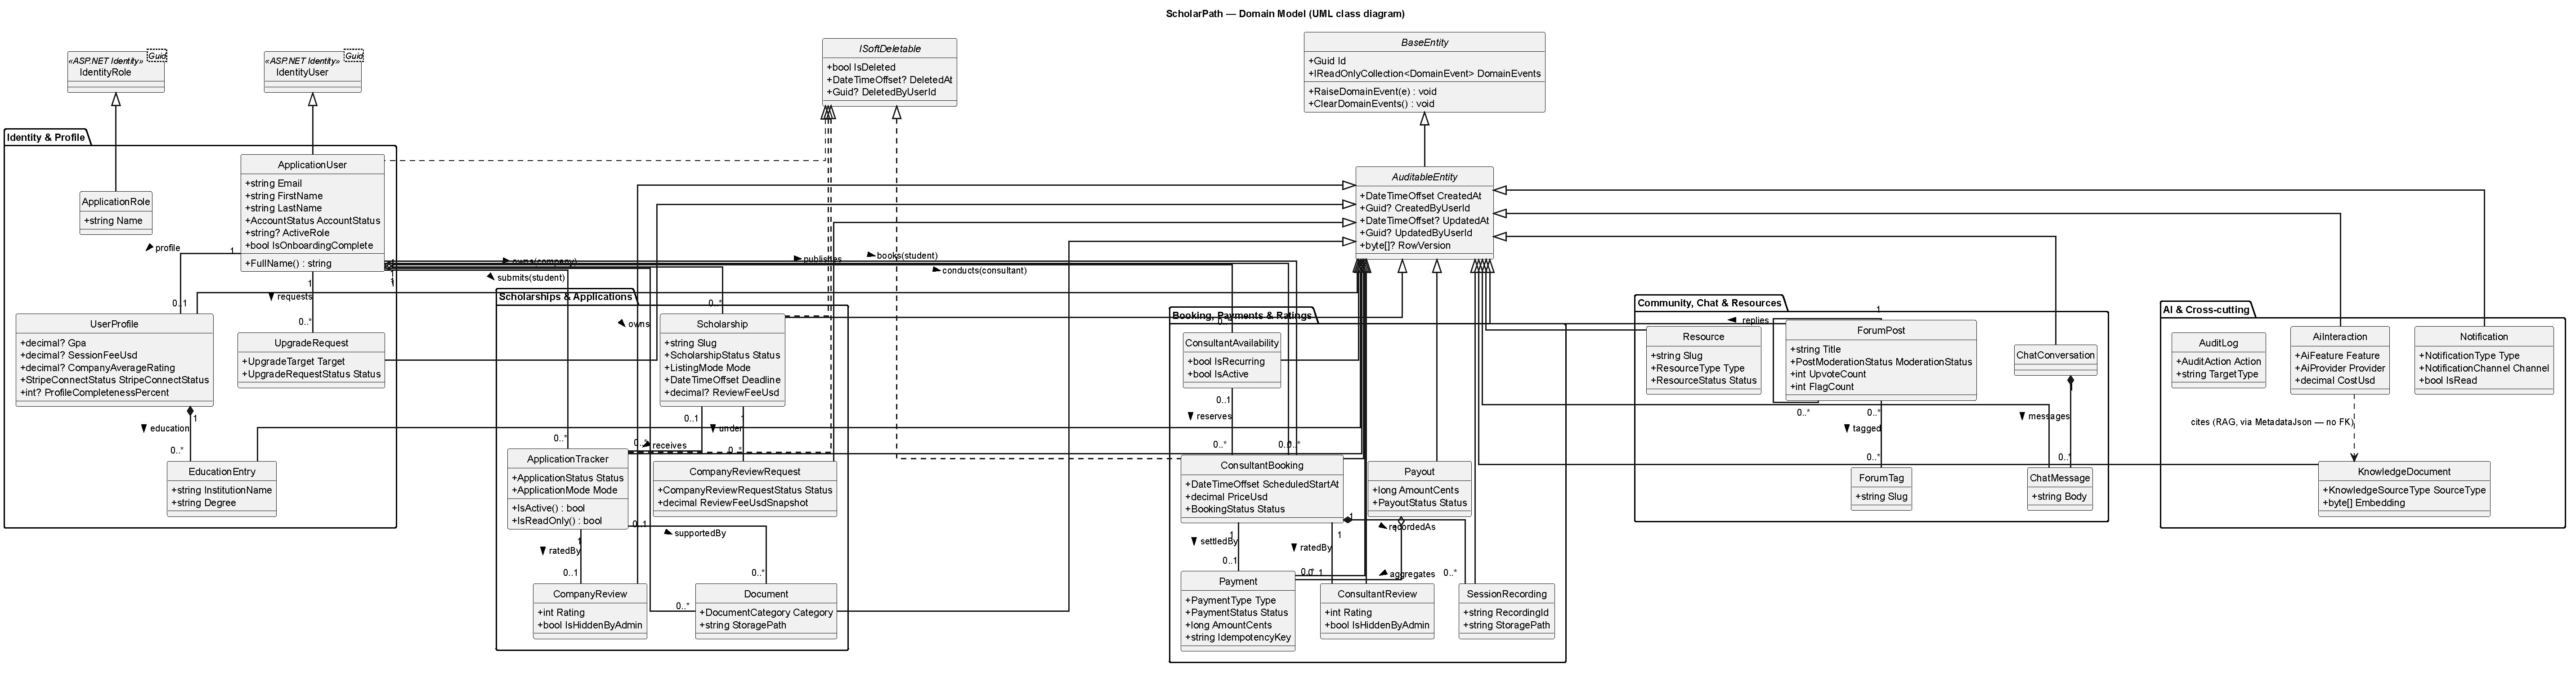
\includegraphics[width=\linewidth,height=0.82\textheight,keepaspectratio]{ScholarPath_Domain_Model.pdf}
\caption{ScholarPath full UML domain model: base types, identity, and every
business cluster with their associations.}\label{fig:domain}
\end{figure}

\subsection{Base types}

\begin{figure}[H]\centering
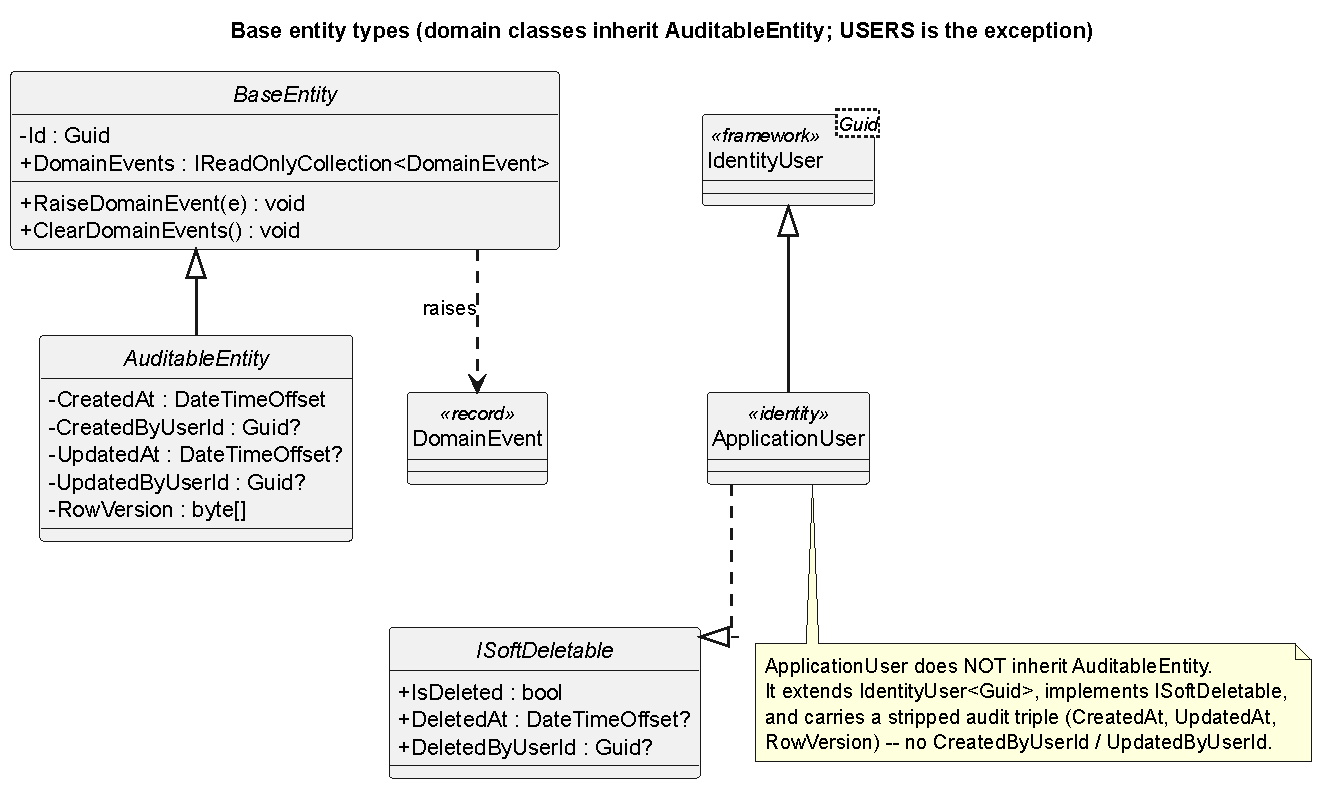
\includegraphics[width=\linewidth,height=0.82\textheight,keepaspectratio]{Class_Base_Types.pdf}
\caption{The inheritance foundation: \texttt{BaseEntity} $\rightarrow$
\texttt{AuditableEntity}, the \texttt{ISoftDeletable} interface, and the ASP.NET
Identity bases.}\label{fig:base}
\end{figure}

This figure isolates the foundation described in Section~2. It shows
\texttt{BaseEntity} as the abstract root, \texttt{AuditableEntity} generalizing
it with the audit/concurrency fields, the \texttt{ISoftDeletable} interface, and
the two ASP.NET Identity base classes that \texttt{ApplicationUser} and
\texttt{ApplicationRole} extend. Every subsequent cluster figure assumes these
parents and omits redundant audit columns to keep each diagram readable.

\subsection{Identity \& Profile}

\begin{figure}[H]\centering
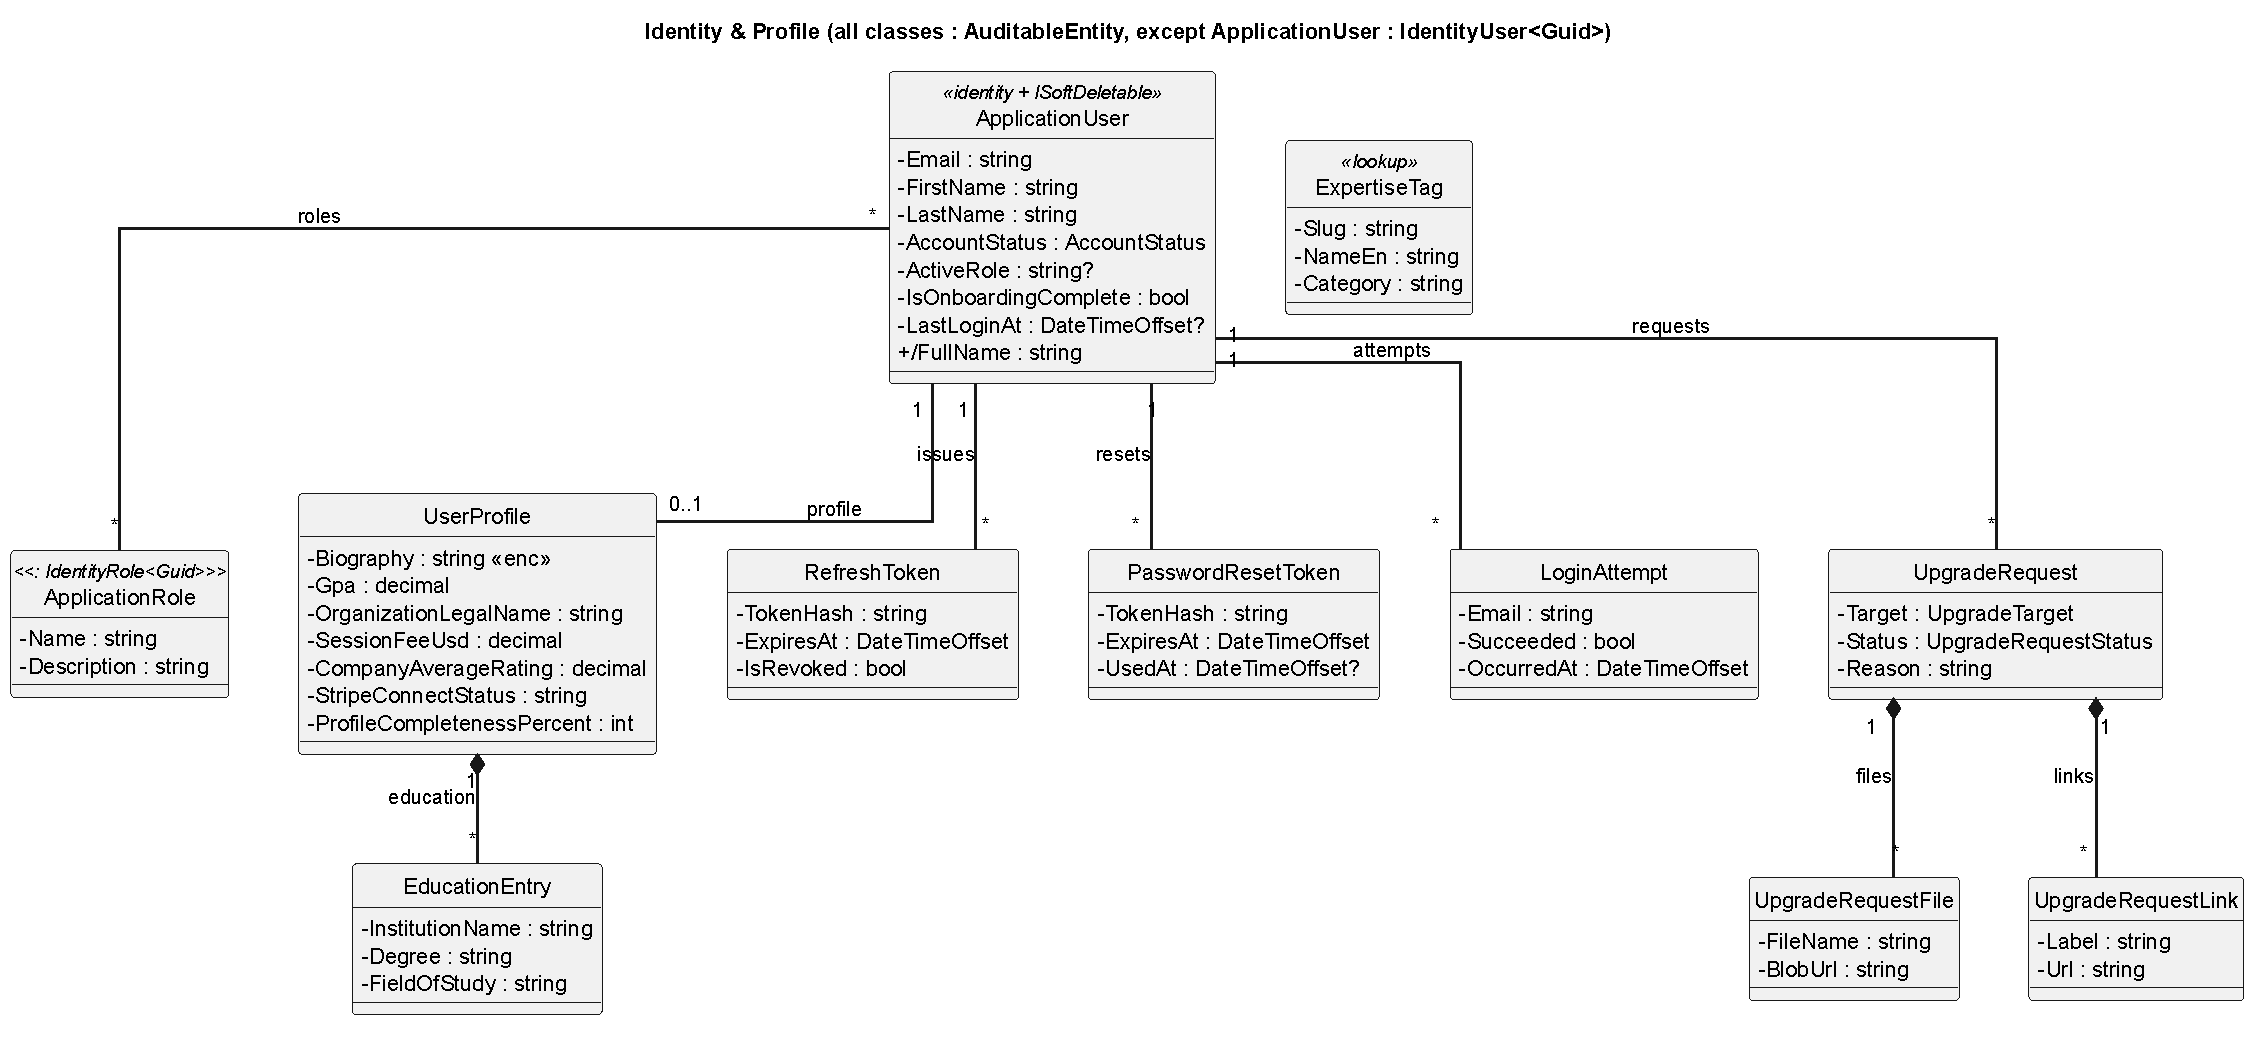
\includegraphics[width=\linewidth,height=0.82\textheight,keepaspectratio]{Class_Identity_Profile.pdf}
\caption{Identity and profile cluster: \texttt{ApplicationUser},
\texttt{ApplicationRole}, \texttt{UserProfile}, and \texttt{EducationEntry}.}
\label{fig:identity}
\end{figure}

An \texttt{ApplicationUser} has at most one \texttt{UserProfile}
(\texttt{1 --> 0..1}), which holds the rich, role-specific attributes:
\texttt{Gpa}, \texttt{SessionFeeUsd}, \texttt{CompanyAverageRating}, the
\texttt{StripeConnectStatus}, and a computed \texttt{ProfileCompletenessPercent}.
The relationship between \texttt{UserProfile} and \texttt{EducationEntry} is a
\textbf{composition} (\texttt{UserProfile *-- EducationEntry}): an education
record describes the academic history of exactly one profile and has no
independent meaning, so it is owned by --- and deleted with --- its profile.

\subsection{Scholarships \& Applications}

\begin{figure}[H]\centering
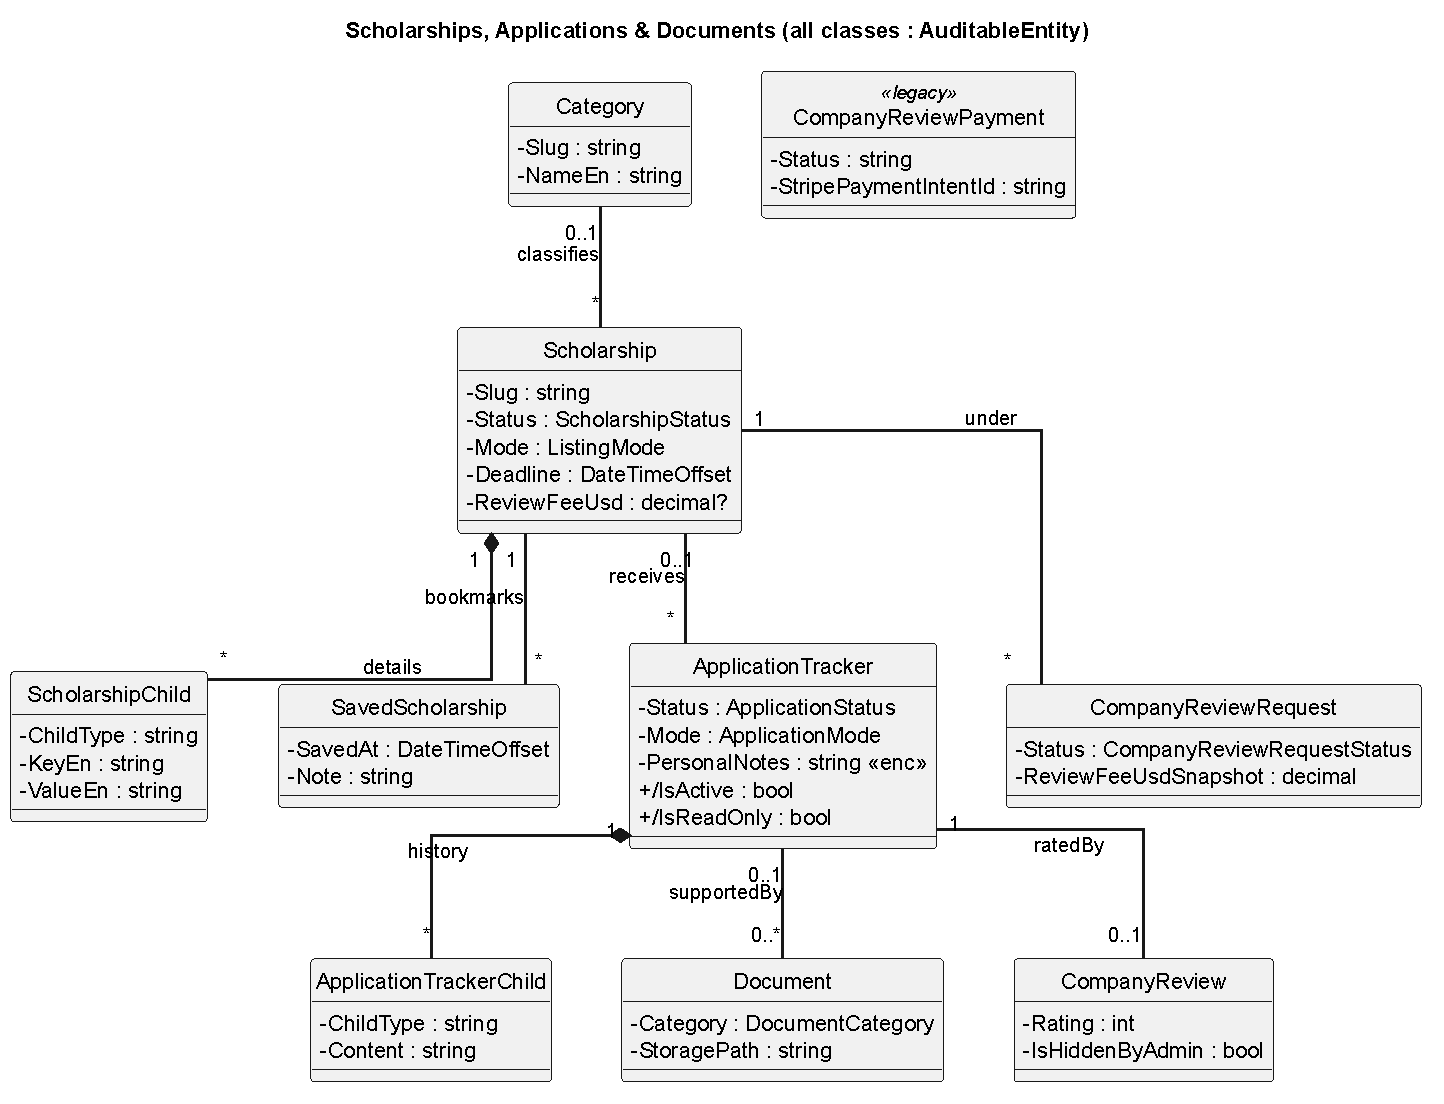
\includegraphics[width=\linewidth,height=0.82\textheight,keepaspectratio]{Class_Scholarships_Applications.pdf}
\caption{Scholarships and applications cluster: \texttt{Scholarship},
\texttt{ApplicationTracker}, \texttt{Document}, and the company-review path.}
\label{fig:scholar}
\end{figure}

A \texttt{Scholarship} (with its \texttt{Slug}, \texttt{Status}, listing
\texttt{Mode}, \texttt{Deadline}, and optional \texttt{ReviewFeeUsd}) is owned by
at most one company user --- modelled as an \emph{aggregation}
(\texttt{ApplicationUser o-- Scholarship}) because a scholarship can outlive a
change of ownership and is not destroyed merely because the listing is
re-assigned. A student submits many \texttt{ApplicationTracker} rows, each
carrying an \texttt{ApplicationStatus}, an \texttt{ApplicationMode}, a
\texttt{SubmittedAt} timestamp, and behaviour such as \texttt{IsActive()} and
\texttt{IsReadOnly()} that governs the state machine.

A point worth emphasising for the committee: \texttt{Document} is associated
with an \texttt{ApplicationTracker} as \textbf{one-to-many}
(\texttt{ApplicationTracker "0..1" --> "*" Document}), \emph{not} as an optional
single attachment. One application is supported by many documents (transcript,
recommendation letters, essays, and so on), and each document is also owned by
the uploading \texttt{ApplicationUser}. The company-review path adds
\texttt{CompanyReviewRequest} (raised by a student against a scholarship, with a
\texttt{ReviewFeeUsdSnapshot}) and the resulting \texttt{CompanyReview} rating
that an \texttt{ApplicationTracker} may receive.

\subsection{Booking, Payments \& Ratings}

\begin{figure}[H]\centering
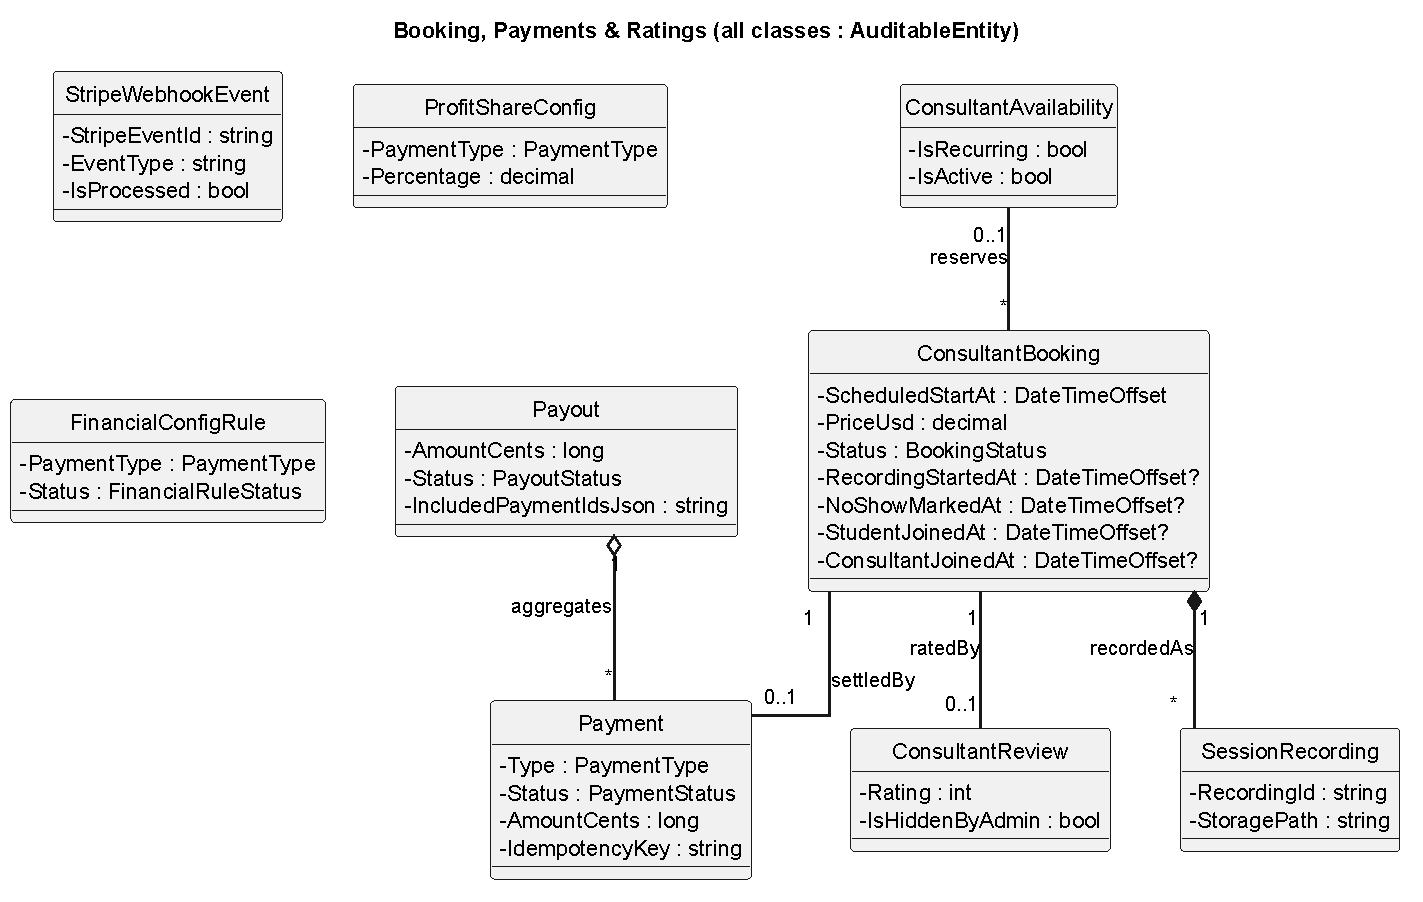
\includegraphics[width=\linewidth,height=0.82\textheight,keepaspectratio]{Class_Booking_Payments_Ratings.pdf}
\caption{Consultant booking, payments, payouts, ratings, and session
recordings.}\label{fig:booking}
\end{figure}

A consultant publishes \texttt{ConsultantAvailability} slots (aggregation: a
slot can be deactivated yet retained for history), which a student reserves as a
\texttt{ConsultantBooking} carrying \texttt{ScheduledStartAt},
\texttt{DurationMinutes}, \texttt{PriceUsd}, a \texttt{BookingStatus}, and a
no-show flag. The same user class appears at both ends of the booking ---
once as the booking student, once as the conducting consultant --- which is why
role names on the associations matter. A booking is settled by at most one
\texttt{Payment} and rated by at most one \texttt{ConsultantReview}.

Two modelling choices are notable. First, \texttt{ConsultantBooking *-- SessionRecording}
is a \textbf{composition}: a recording has no life outside the booking that
produced it, so it is destroyed with the booking. Second,
\texttt{Payout o-- Payment} is an \textbf{aggregation}: a payout batches many
already-existing payments and the payments survive the payout record. As Part~3
noted, the \texttt{Payment}/\texttt{Payout} links are drawn as UML associations
but are \emph{application-enforced} rather than backed by database foreign keys.
The \texttt{Payment} class also carries the money-split fields
(\texttt{AmountCents}, \texttt{ProfitShareAmountCents}, \texttt{PayeeAmountCents})
and an \texttt{IdempotencyKey} that makes retries safe.

\subsection{Community \& Chat}

\begin{figure}[H]\centering
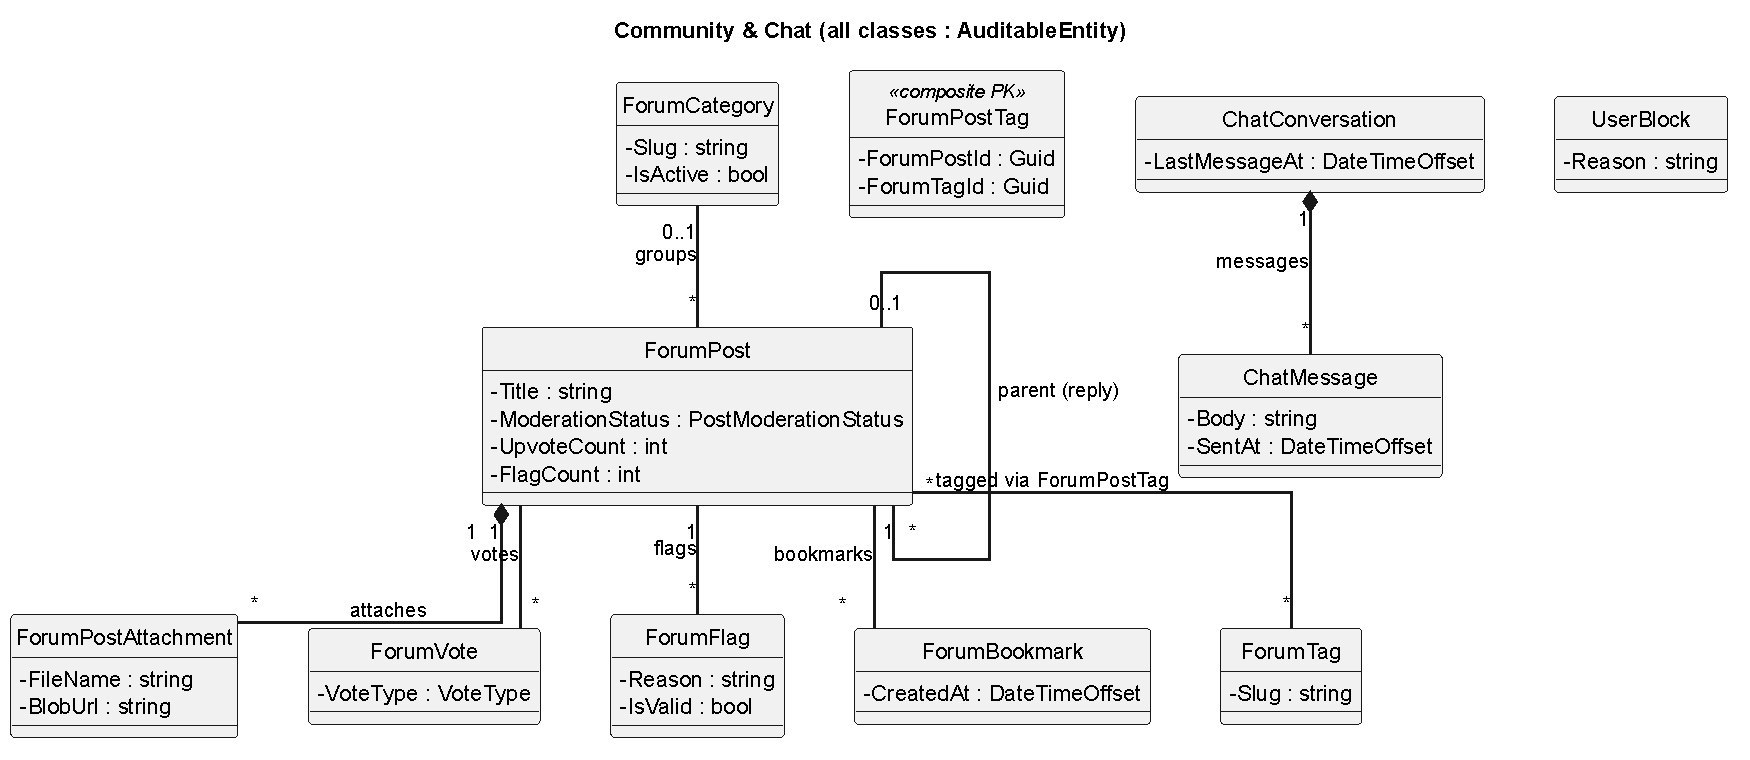
\includegraphics[width=\linewidth,height=0.82\textheight,keepaspectratio]{Class_Community_Chat.pdf}
\caption{Community forum (posts, votes, flags, tags) and direct chat
(conversations and messages).}\label{fig:community}
\end{figure}

A \texttt{ForumPost} carries a self-association to model threaded replies
(\texttt{ForumPost "1" --> "0..1" ForumPost : parent}). Its \texttt{ForumVote}
and \texttt{ForumFlag} children are \textbf{compositions} --- a vote or a flag
is meaningless without the post it targets. Tagging is a many-to-many resolved
through the \texttt{ForumPostTag} \texttt{<<junction>>} class, mirroring the
bridge table from Part~3. On the chat side, a \texttt{ChatConversation} is a
\textbf{composition} of \texttt{ChatMessage} objects
(\texttt{ChatConversation *-- ChatMessage}): messages belong wholly to their
conversation and are removed with it.

\subsection{Resources \& Notifications}

\begin{figure}[H]\centering
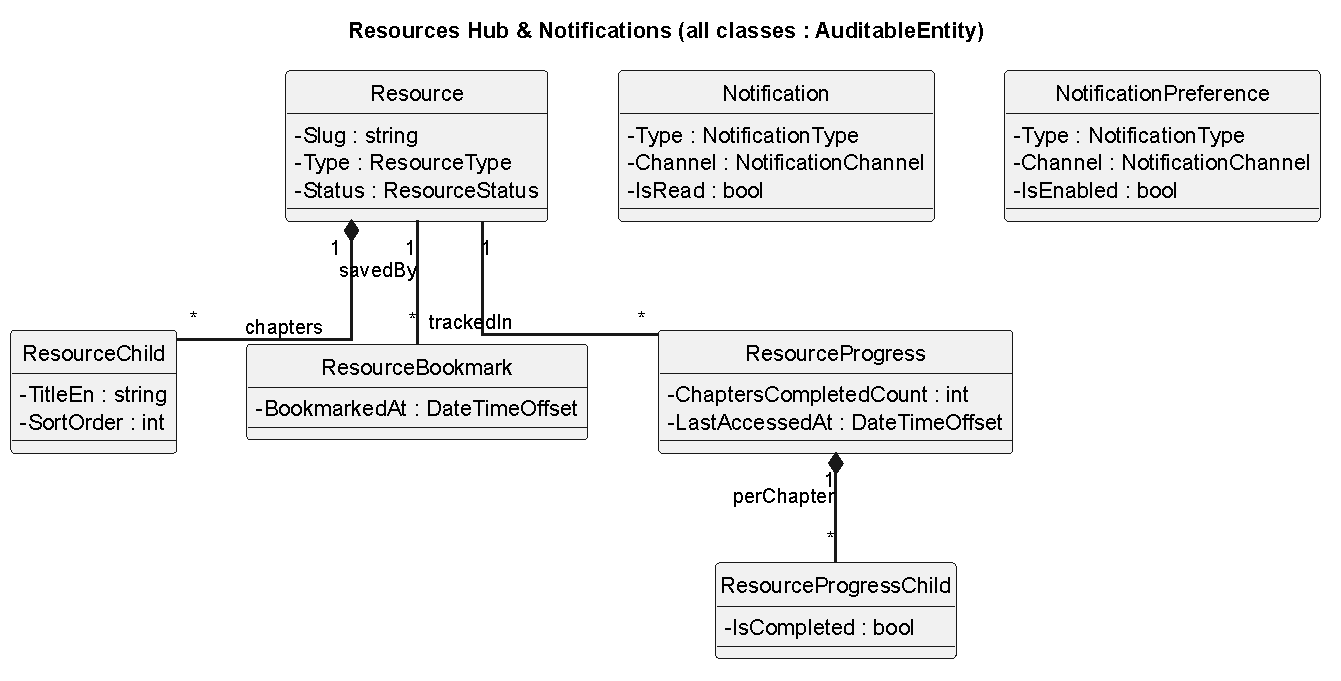
\includegraphics[width=\linewidth,height=0.82\textheight,keepaspectratio]{Class_Resources_Notifications.pdf}
\caption{Learning resources (with their chapters and per-user progress) and the
notification entity.}\label{fig:resources}
\end{figure}

A \texttt{Resource} (\texttt{Slug}, \texttt{Type}, \texttt{Status},
\texttt{AuthorRole}) is composed of ordered \texttt{ResourceChild} chapters
(\texttt{Resource *-- ResourceChild}) and is tracked by many
\texttt{ResourceProgress} rows, one per learner, recording
\texttt{ChaptersCompletedCount}. \texttt{Notification} captures a typed,
multi-channel alert (\texttt{NotificationType}, \texttt{NotificationChannel},
\texttt{IsRead}) and is the entity written by the notification dispatcher
described in Section~4.

\subsection{AI Platform}

\begin{figure}[H]\centering
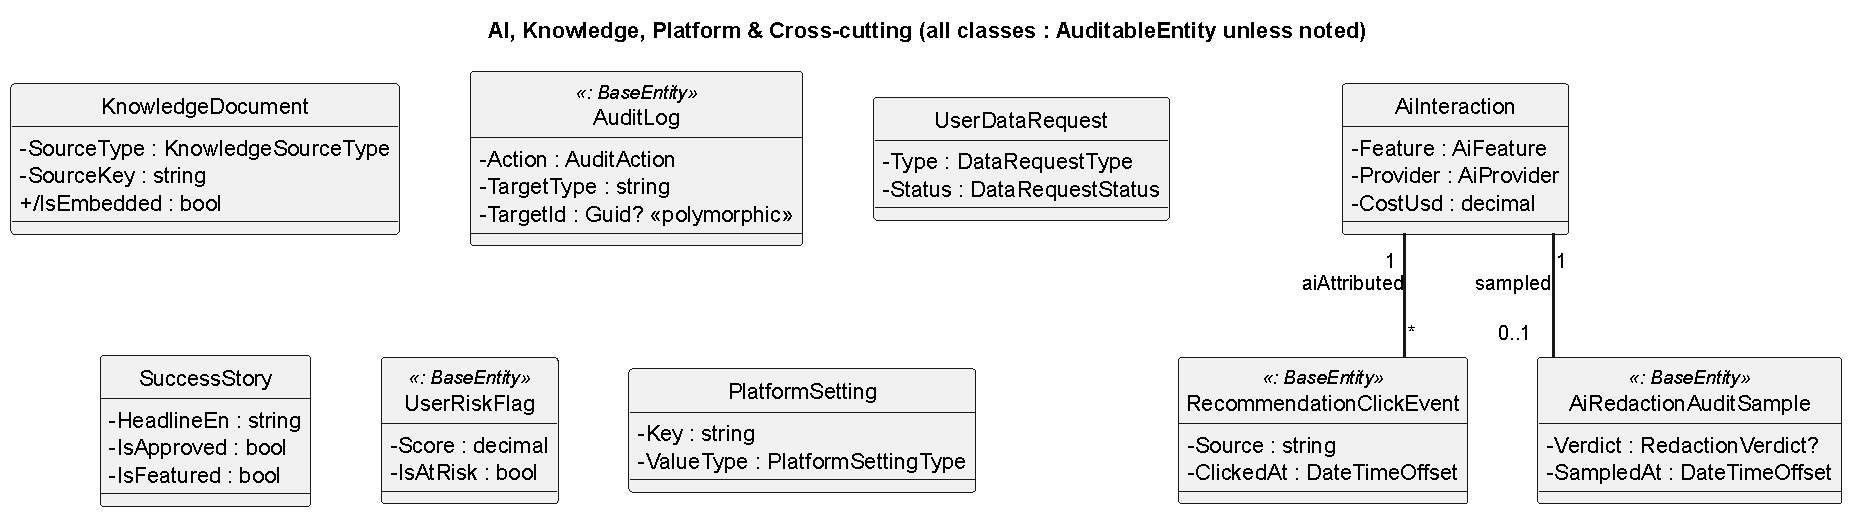
\includegraphics[width=\linewidth,height=0.82\textheight,keepaspectratio]{Class_AI_Platform.pdf}
\caption{AI platform entities: \texttt{AiInteraction} usage records and the
\texttt{KnowledgeDocument} RAG corpus.}\label{fig:ai}
\end{figure}

\texttt{AiInteraction} logs every model call --- the \texttt{AiFeature} invoked,
the \texttt{AiProvider} used, the \texttt{CostUsd}, and token counts such as
\texttt{PromptTokens} --- giving the platform full cost and audit visibility.
\texttt{KnowledgeDocument} is the Retrieval-Augmented Generation (RAG) corpus,
storing a \texttt{SourceType}, a vector \texttt{Embedding}, and a
\texttt{ContentHash} for deduplication. The link
\texttt{AiInteraction ..> KnowledgeDocument} is a \emph{dependency}, not an
association with a foreign key: an interaction cites the documents it retrieved
through a \texttt{MetadataJson} field rather than a relational reference, which
is why Part~3's schema shows no FK between them.

\section{Clean Architecture: The Ports-and-Adapters Seam}

\subsection{Ports defined by the Application layer}

ScholarPath follows Clean Architecture: dependencies point inward
(\texttt{API} $\rightarrow$ \texttt{Application} $\rightarrow$ \texttt{Domain};
\texttt{Infrastructure} $\rightarrow$ \texttt{Application}/\texttt{Domain}). The
crucial design device is the \emph{port}: the Application layer declares a set of
interfaces describing \emph{what} it needs, with no knowledge of \emph{how} those
needs are met. These ports include \texttt{IAiService},
\texttt{IEmbeddingService}, \texttt{IStripeService}, \texttt{IMeetingService},
\texttt{IEmailService}, \texttt{IBlobStorageService}, \texttt{IFileScanService},
\texttt{IFieldEncryptionService}, \texttt{IPowerBiService},
\texttt{IEventPublisher}, \texttt{INotificationDispatcher}, the realtime
notifiers (\texttt{IChatRealtimeNotifier}, \texttt{ICommunityRealtimeNotifier}),
and the persistence port \texttt{IApplicationDbContext}. Because use-cases depend
only on these abstractions, the business logic is fully unit-testable with
in-memory fakes.

\subsection{Adapters provided by the Infrastructure layer}

Figure~\ref{fig:ports} shows the seam: each port (interface) on the left is
\emph{realized} by one or more adapters on the right, and the concrete adapter is
chosen at start-up by dependency injection and configuration (for example
\texttt{Ai\_\_Provider} and the hosting environment). This is what lets
ScholarPath run fully offline in development yet hit real Azure services in
production without changing a single line of application code.

\begin{figure}[H]\centering
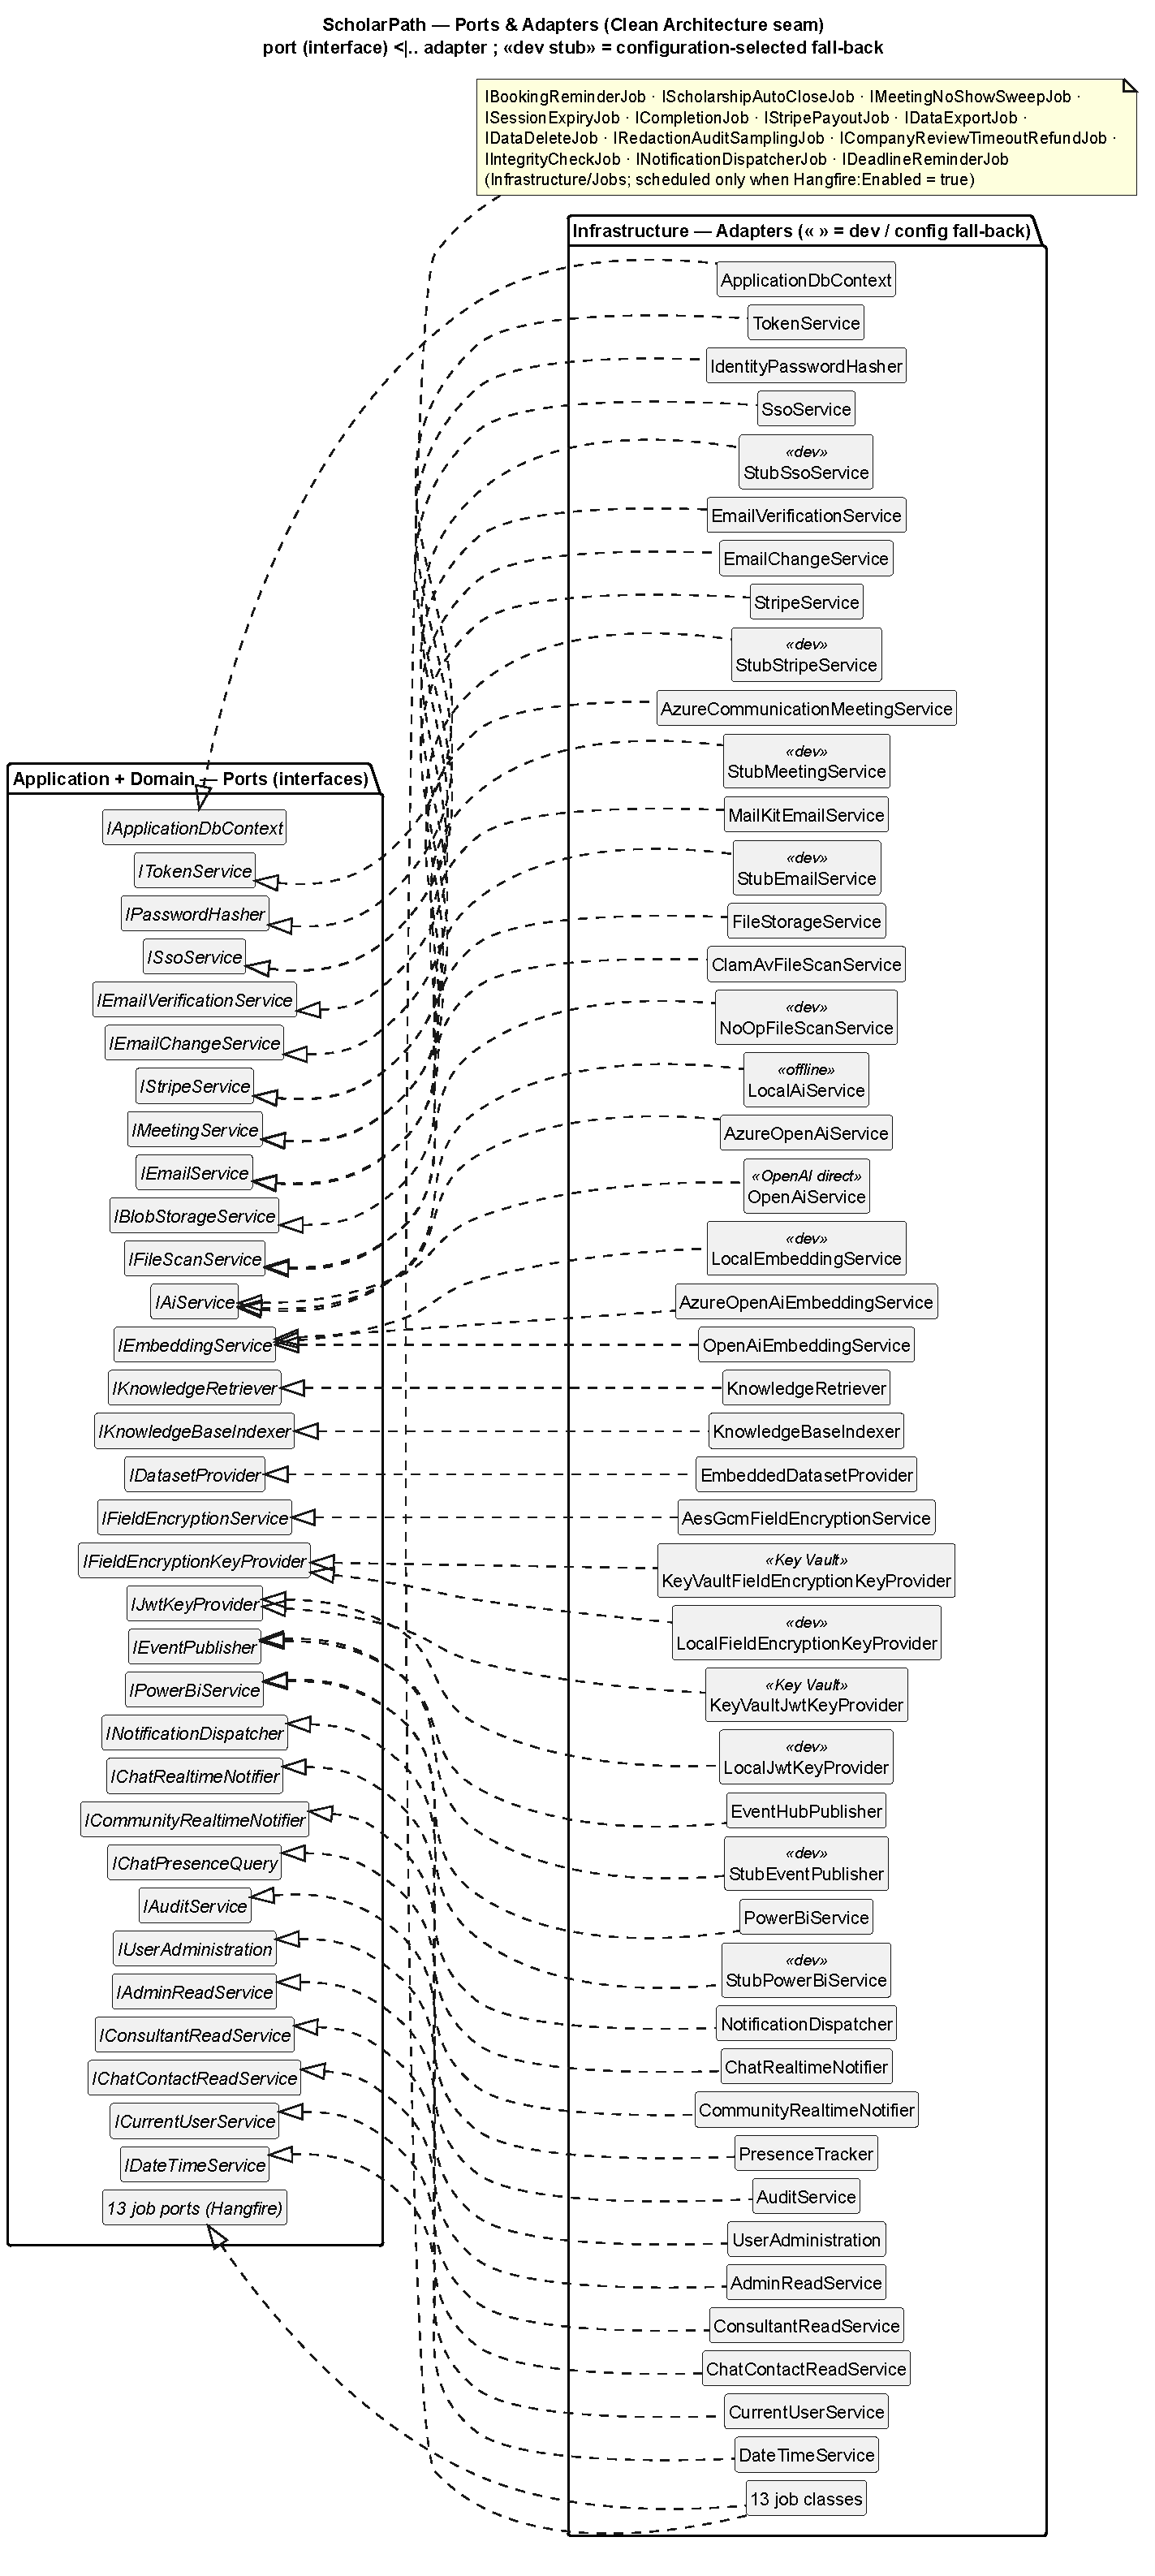
\includegraphics[width=\linewidth,height=0.82\textheight,keepaspectratio]{ScholarPath_Ports_Adapters.pdf}
\caption{Ports (Application interfaces) realized by Infrastructure adapters,
selected by configuration; every port has a production adapter and a dev
stub/local fallback.}\label{fig:ports}
\end{figure}

Table~\ref{tab:adapters} lists the principal port-to-adapter realizations.
Notably, the AI port has three adapters --- two production providers and one
local fallback --- selected purely by configuration.

\begin{table}[H]\centering
\caption{Ports and their realizing adapters (production and dev fallback).}
\label{tab:adapters}
\small
\begin{tabular}{@{}l l l@{}}
\toprule
\textbf{Port (Application)} & \textbf{Production adapter} & \textbf{Dev fallback} \\
\midrule
\texttt{IApplicationDbContext} & \texttt{ApplicationDbContext} (EF Core) & --- \\
\texttt{IAiService} & \texttt{AzureOpenAiService} / \texttt{OpenAiService} & \texttt{LocalAiService} \\
\texttt{IEmbeddingService} & \texttt{AzureOpenAiEmbeddingService} / \texttt{OpenAiEmbeddingService} & \texttt{LocalEmbeddingService} \\
\texttt{IStripeService} & \texttt{StripeService} & \texttt{StubStripeService} \\
\texttt{IMeetingService} & \texttt{AzureCommunicationMeetingService} & \texttt{StubMeetingService} \\
\texttt{IEmailService} & \texttt{MailKitEmailService} & \texttt{StubEmailService} \\
\texttt{IBlobStorageService} & \texttt{FileStorageService} (Azure Blob) & Local storage provider \\
\texttt{IFileScanService} & \texttt{ClamAvFileScanService} & \texttt{NoOpFileScanService} \\
\texttt{IFieldEncryptionService} & \texttt{AesGcmFieldEncryptionService} + Key Vault & --- \\
\texttt{IPowerBiService} & \texttt{PowerBiService} & \texttt{StubPowerBiService} \\
\texttt{IEventPublisher} & \texttt{EventHubPublisher} & \texttt{StubEventPublisher} \\
\texttt{INotificationDispatcher} & \texttt{NotificationDispatcher} & --- \\
\bottomrule
\end{tabular}
\end{table}

The realization relationship in UML (\texttt{Interface <|.. Class}) is exactly
the right glyph for this seam. For instance:

\begin{lstlisting}[language=, caption={Realization of the AI port by three interchangeable adapters.}]
IAiService          <|.. AzureOpenAiService   // Ai__Provider=AzureOpenAi
IAiService          <|.. OpenAiService         // Ai__Provider=OpenAi
IAiService          <|.. LocalAiService        // dev / offline fallback
IEmbeddingService   <|.. AzureOpenAiEmbeddingService
IEmbeddingService   <|.. OpenAiEmbeddingService
IEmbeddingService   <|.. LocalEmbeddingService
IStripeService      <|.. StripeService
IMeetingService     <|.. AzureCommunicationMeetingService
\end{lstlisting}

The production adapters integrate Azure OpenAI (chat + embeddings, with an
OpenAI-direct alternative), Stripe (PaymentIntents, capture, refund, Connect
payouts), Azure Communication Services (video rooms and recording), MailKit over
SMTP, ClamAV for malware scanning of uploads, AES-GCM field encryption keyed by
Azure Key Vault, Azure Event Hub feeding Power BI, and the
\texttt{NotificationDispatcher} that fans an alert out to the
\texttt{Notifications} table, e-mail, and SignalR simultaneously. Every one of
these has a dev-time stub or local fallback so the platform behaves identically
offline. The wider deployment topology of these integrations is covered in the
companion component and deployment diagram.

\section{Conclusion}

This object model is the executable form of the relational schema produced in
Part~3. The tables of the Relational Mapping document become the C\# domain
classes presented here; the foreign keys become typed associations with explicit
multiplicities; the repeated audit columns are explained by the
\texttt{BaseEntity} $\rightarrow$ \texttt{AuditableEntity} inheritance; the
soft-delete columns are the realization of \texttt{ISoftDeletable}; and the bridge
tables become \texttt{<<junction>>} classes. Two design decisions deserve a final
note for the committee: \texttt{ApplicationUser} extends ASP.NET
\texttt{IdentityUser<Guid>} rather than the domain base, and \texttt{Document} is
a one-to-many child of \texttt{ApplicationTracker} rather than an optional single
attachment. Layered on top, the ports-and-adapters seam keeps the entire domain
and application logic independent of any external vendor, which is the property
that makes ScholarPath both testable and portable. Together with the ERD, EERD,
and Relational Mapping documents that precede it, this completes a single
unbroken line from conceptual model to running object-oriented system.

\end{document}
